Long before cities, agriculture, written records, or modern technology, humans lived in small groups navigating an uncertain world. Survival depended not only on individual intelligence but also on the ability to act collectively. Groups hunted, gathered food, protected offspring, shared resources, and learned from one another. Many accounts of human social evolution emphasise cooperation and social bonding as important pressures shaping communication~\cite{tomasello2008origins,dunbar1996grooming}.

As human societies became larger and their activities more complex, the demands placed on communication also increased. Groups needed to remember where resources had previously been found, teach tool-making techniques, coordinate hunting strategies, divide responsibilities, and adapt plans when circumstances changed. Improved communication was needed to refer to distant locations, future actions, past experiences, hidden constraints, and the intentions of other individuals~\cite{clark1996usinglanguage,tomasello2008origins}.

Language likely emerged gradually alongside human social and cognitive evolution rather than appearing as a fully formed system~\cite{johansson2005origins}. Simple signals became richer, more structured, and more expressive. Sounds, gestures, and shared symbols acquired stable meanings that enabled more sophisticated interactions. As collective activities became more demanding, communication evolved to support them. At the same time, social and organisational pressures favoured further advances in communication~\cite{tomasello2008origins,dunbar1996grooming}.

This co-evolution produced a feedback loop in which improved communication supported larger groups, specialised roles, more effective teaching, and advanced planning, while these social developments encouraged further refinements in communication. Many accounts of language evolution consequently view language and collective action as deeply intertwined phenomena. Language is often associated with shared intentionality, social organisation, cooperation, and the practical demands of acting together in complex environments~\cite{clark1996usinglanguage,tomasello2008origins,dunbar1996grooming,johansson2005origins}.

The development of written language further extended these capabilities. Knowledge, procedures, plans, and experiences could now persist beyond immediate interactions and be shared across larger groups and across generations~\cite{fischer2004history}. Human societies accumulated large bodies of recorded information, creating new opportunities for learning, coordination, and collective problem-solving.

The growth of written language and, later, digital information created an unprecedented repository of human knowledge~\cite{fischer2004history}. Books, articles, manuals, conversations, reports, and countless other forms of written communication captured facts, goals, plans, instructions, explanations, negotiations, and other artefacts of human problem-solving. As digital text collections expanded, researchers began developing computational methods capable of modelling and generating language automatically~\cite{jurafsky2025speech}.

Early computational language models represented language through statistical relationships between words and phrases~\cite{jurafsky2025speech}. Neural probabilistic language models later showed how such relationships could be learned through distributed representations~\cite{bengio2003neural}, and word-embedding methods scaled distributed representations to large text corpora~\cite{mikolov2013distributed}. The introduction of transformer-based architectures marked a significant advance in language modelling~\cite{vaswani2017attention}. Together, these developments contributed to the emergence of large-scale foundation models trained on broad data collections~\cite{bommasani2021foundation}.

Modern large language models (LLMs) are trained on extensive collections of human-generated language~\cite{brown2020language,bommasani2021foundation}. Unlike systems based on manually encoded rules or task-specific reasoning procedures, they acquire behaviour from statistical patterns in examples contained within their training data~\cite{brown2020language,bommasani2021foundation}. This exposes the models to many forms of human activity expressed through language, including planning, instruction following, explanation, negotiation, coordination, and collaborative problem-solving~\cite{brown2020language,bommasani2021foundation}.

Although LLMs are fundamentally trained to predict the next token in a sequence, recent studies suggest that they can exhibit capabilities extending beyond simple text completion~\cite{bommasani2021foundation,jurafsky2025speech}. Under suitable prompting strategies, language models have been shown to generate plausible plans~\cite{huang2022lmp}, decompose complex tasks into intermediate sub-goals~\cite{wang2023planandsolve}, reason over sequences of actions~\cite{yao2022react}, and explore alternative reasoning paths when constraints or objectives change~\cite{yao2023tree}. These observations have motivated growing interest in the use of language models as components of decision-making and planning systems rather than solely as tools for text generation.

A natural question follows: if language evolved alongside sophisticated forms of collective action, and modern language models learn patterns from descriptions of goals, plans, responsibilities, and constraints, could such models contribute to decision-making in situations where multiple entities must work together towards a shared objective? The present thesis investigates this possibility in the context of multi-agent systems.

Many real-world problems cannot be solved effectively by a single decision-making entity. Instead, they involve multiple entities that must operate within a shared environment while pursuing individual or collective objectives. In artificial intelligence and robotics, such entities are commonly referred to as agents. An agent is a system that perceives its environment and selects actions based on those perceptions~\cite{russell2021}. When multiple agents operate within the same environment, the resulting system is commonly referred to as a multi-agent system (MAS)~\cite{wooldridge2009}.

As the number of agents increases, decision-making becomes more challenging. Agents may compete for resources, interfere with one another, require access to shared information, or depend on each other to complete tasks. Consequently, the ability to organise and align the actions of multiple agents becomes a central concern in multi-agent and multi-robot systems~\cite{yan2013mrscoordination}.

Researchers have proposed several concepts to describe different forms of collective behaviour among agents. Terms such as coordination, cooperation, and collaboration are often used throughout the literature, although their meanings are not always consistent. In some cases the terms are used interchangeably, while in others they describe distinct levels of interaction between agents. Because these concepts are central to the present thesis, the following definitions are adopted.

In this thesis, \emph{coordination} refers to arranging actions, timing, information, or resource usage so that agents do not interfere with one another and can make progress towards their objectives. \emph{Cooperation} refers to situations in which agents pursue a shared objective, even if their individual actions are not tightly interdependent. \emph{Collaboration} is used for the stronger case where agents depend on one another to complete a task and where progress requires explicit interaction between different roles or capabilities. These distinctions are important because the literature does not always use the terms consistently, particularly across multi-agent systems, multi-robot systems, and human teamwork~\cite{yan2013mrscoordination}.

A particularly important class of multi-agent systems is the multi-robot system (MRS), where the agents are physical robots operating within a shared environment. Multi-robot systems have been studied in domains such as manufacturing, logistics, exploration, transportation, and search-and-rescue operations~\cite{yan2013mrscoordination}. As in human teams, effective performance often depends on the capabilities of individual agents and their ability to coordinate and collaborate with one another.


Multi-robot systems appear in many domains, including manufacturing, transportation, agriculture, exploration, and logistics. Among these, warehouse logistics has received particular attention due to the rapid growth of e-commerce and the increasing demand for fast order fulfilment. Global e-commerce continues to expand and constitutes an increasingly important component of the digital economy, placing substantial pressure on warehouse operations, fulfilment networks, and inventory management systems~\cite{unctad2024digital}. As a result, improving warehouse efficiency has become both an important industrial objective and an active area of research.
Warehouse environments are also particularly relevant from a multi-agent systems perspective. Fulfilling customer orders requires the interaction of multiple resources, including storage locations, transportation systems, workstations, inventory-management processes, and, increasingly, autonomous robots. These resources operate under shared constraints and must be coordinated to ensure efficient order fulfilment, making warehouse logistics a practical and representative domain for studying multi-agent and multi-robot decision-making~\cite{bartholdi2019warehouse}.

Consider a customer placing an online order. The requested item may be stored on a shelf among thousands of products distributed throughout a warehouse. To fulfil the order, the item must be located, retrieved from storage, transported to a picking or packing area, prepared for shipment, and eventually dispatched for delivery. Throughout this process, multiple resources must interact efficiently to ensure that the correct item reaches the customer on time~\cite{bartholdi2019warehouse}.

\begin{figure}[H]
    \centering
    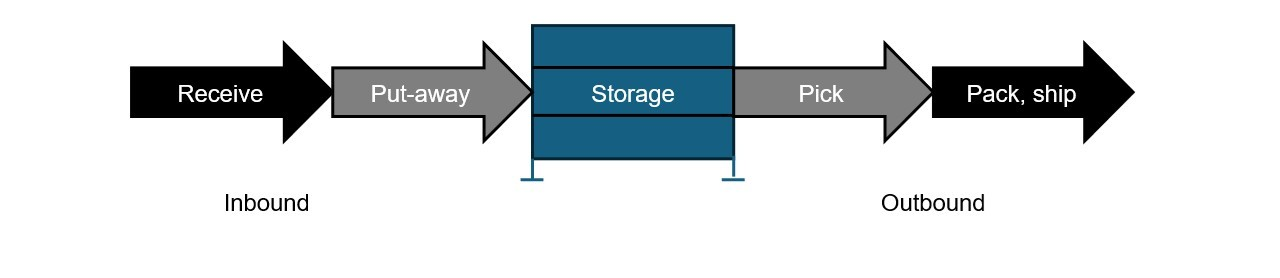
\includegraphics[width=0.95\textwidth]{figures/WarehouseFlowcr.jpg}
    \caption{Overview of the warehouse goods flow.}
    \label{fig:warehouse_order_fulfilment}
\end{figure}


Warehousing is a broad discipline with its own terminology and operational practices. This thesis introduces only the concepts necessary to understand the experimental environment; a more comprehensive discussion of warehouse operations can be found in Bartholdi and Hackman~\cite{bartholdi2019warehouse}.

In a typical warehouse, products are stored in designated storage locations such as shelves, racks, bins, or movable storage units. Customer requests are represented as orders that specify which items must be retrieved. The process of retrieving requested items from storage is commonly referred to as picking. Depending on the warehouse design, picked items may be transported to packing stations, where orders are prepared for shipment, before being sent to delivery or dispatch stations for onward transportation~\cite{bartholdi2019warehouse,dekoster2007design}.
\begin{figure}[H]
    \centering
    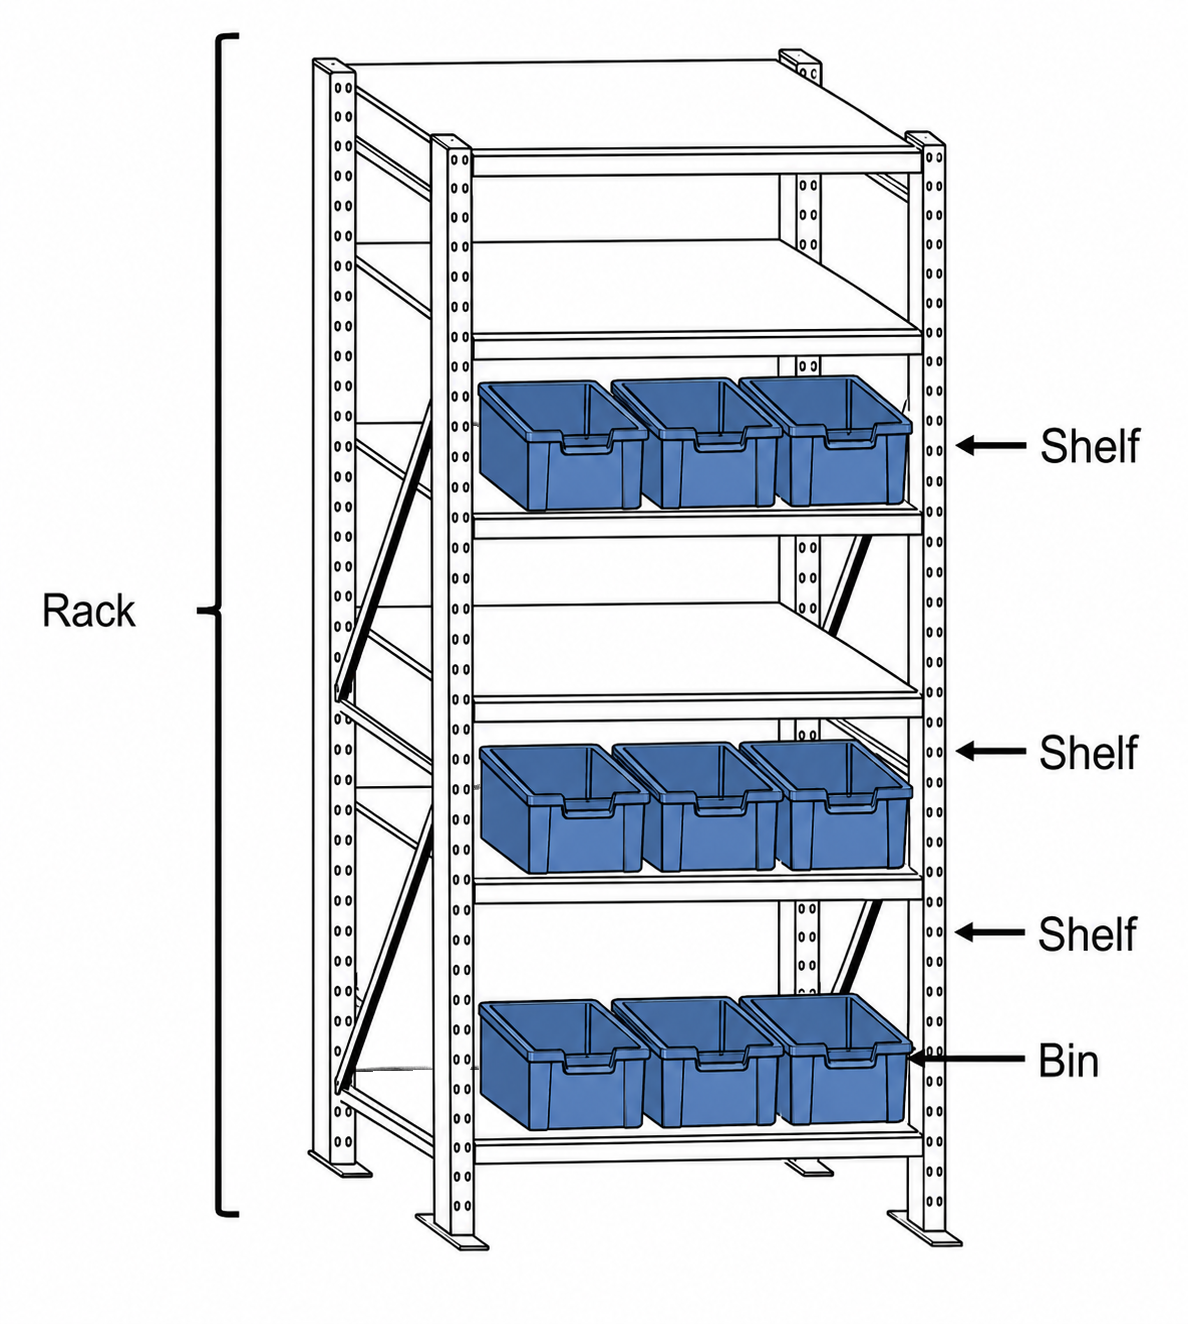
\includegraphics[width=0.95\textwidth]{figures/Rack-shelves-bin.png}
    \caption{Example warehouse storage hierarchy showing a rack composed of multiple shelves and storage bins.}
    \label{fig:warehouse_storage_hierarchy}
\end{figure}
The resources involved in these activities may include human workers, automated storage systems, mobile robots, workstations, and warehouse management software. Together, these components form a workflow whose objective is to fulfil customer orders accurately and efficiently.
Traditionally, warehouses operated according to a person-to-goods paradigm. Human workers travelled through storage aisles to locate and retrieve products. While straightforward to implement, worker travel often represented a significant portion of fulfilment time and operational cost~\cite{dekoster2007design}.

As order volumes increased, particularly with the growth of e-commerce, alternative approaches emerged. In goods-to-person systems, products or storage units are brought to stationary workers instead of requiring workers to travel throughout the warehouse. This reduces travel time but introduces new coordination challenges, since storage units, workstations, and transportation resources must now be scheduled and synchronised effectively~\cite{boysen2019warehousing,barros2021rmfs}.

Robotic warehouse systems emerged as a natural extension of this evolution.
A well-known example is the Kiva-style warehouse system, in which fleets of mobile robots transport inventory pods between storage areas and stationary workstations~\cite{wurman2008coordinating}. 
Unlike traditional racks, which remain fixed in place, inventory pods are movable storage units containing multiple shelves and stored products. Mobile robots navigate beneath these pods, lift them, and transport them to workstations where items can be retrieved~\cite{wurman2008coordinating}.

\begin{figure}[H]
\centering
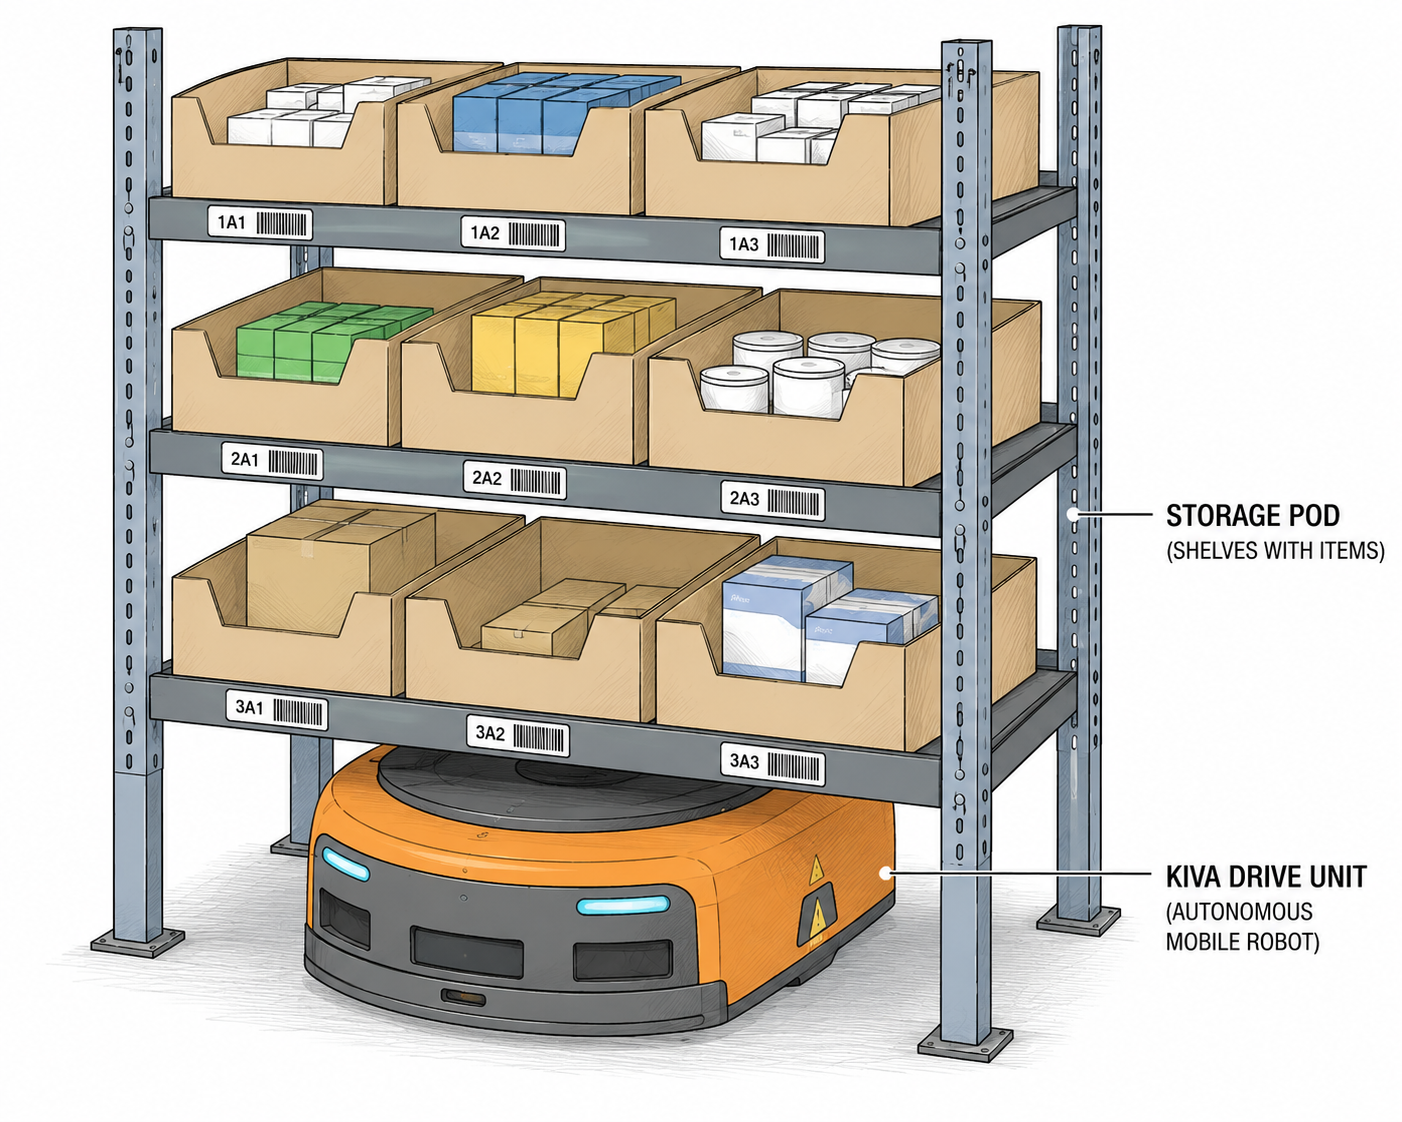
\includegraphics[width=0.95\textwidth]{figures/KivaWarehouse.png}
\caption{Illustration of a Kiva-style inventory pod. The pod contains multiple shelves used for product storage, while a mobile drive unit operates beneath the pod to transport it throughout the warehouse~\cite{wurman2008coordinating}.}
\label{fig:kiva_inventory_pod}
\end{figure}
Rather than asking workers to travel to products, the warehouse brings products to workers. By transporting storage units to stationary workstations, goods-to-person (GTP) systems reduce the need for worker travel and can improve fulfilment efficiency~\cite{wurman2008coordinating}. At the same time, they introduce additional coordination requirements among robots, storage units, and workstations.
The challenge is no longer limited to locating products and fulfilling orders. The warehouse must now determine which storage unit should be moved, which robot should perform the movement, which workstation should receive the requested items, and how shared resources should be allocated when multiple requests compete for attention. As the number of robots, workstations, and orders increases, these decisions become increasingly interdependent~\cite{wurman2008coordinating,barros2021rmfs}.

At this point, warehouse operation becomes a coordination problem. Robots may compete for pathways, storage units, charging stations, or workstations. Tasks may depend on the completion of other tasks. Some activities can be performed independently, while others require multiple resources or specialised roles to interact successfully. The overall performance of the warehouse depends on the capabilities of individual agents and the effectiveness of their coordination~\cite{yan2013mrscoordination}.
Although warehouse logistics provides a useful example, similar challenges appear throughout multi-agent systems. Autonomous vehicle fleets, drone swarms, manufacturing systems, search-and-rescue teams, and service robots must all operate under shared constraints while pursuing common objectives. The underlying challenge is therefore more general than warehouse automation: how can multiple agents make effective decisions while acting within a shared environment?

While coordination is essential in robotic warehouses, many real-world multi-agent systems require a stronger form of interaction. Coordination may be sufficient when agents perform largely independent tasks while sharing resources. Collaboration, however, requires agents to depend on one another in order to achieve a common objective. In such settings, successful task completion depends on the interaction of agents with complementary roles or capabilities~\cite{yan2013mrscoordination,karam2026collaborationmrs}.

Collaborative decision-making introduces additional challenges. Decisions made by one agent may influence the opportunities available to others, while task completion may depend on actions performed by multiple agents. Effective behaviour therefore requires consideration of shared goals, task dependencies, resource constraints, and the expected behaviour of teammates~\cite{karam2026collaborationmrs}. These characteristics make collaborative multi-agent systems an interesting domain for investigating whether language-model-based planning and decision-making can provide useful support.

In many practical multi-agent systems, this interdependence arises because agents possess complementary capabilities rather than identical roles. Progress may therefore depend on interactions between specialised agents that must work together to complete tasks.

Evaluating such decision-making approaches directly in physical robotic systems can be costly, difficult to reproduce, and potentially disruptive to ongoing operations. Changes to coordination or collaboration strategies may affect safety, productivity, equipment utilisation, and interactions between agents operating within the environment. Consequently, simulation has become a widely adopted methodology for studying multi-agent and multi-robot systems~\cite{papoudakis2021benchmarking,krnjaic2024warehouse}.


Simulation environments provide controlled and repeatable conditions in which task distributions, agent capabilities, resource constraints, and environmental characteristics can be varied systematically. This enables researchers to compare different approaches under identical conditions before considering deployment in physical systems.


The growing adoption of simulation has led to the development of standardised benchmark environments. Frameworks such as OpenAI Gym and its successor Gymnasium provide common interfaces that support reproducible experimentation across a wide range of reinforcement-learning and decision-making problems~\cite{brockman2016gym,towers2024gymnasium}.
Warehouse-inspired benchmark environments have become particularly popular because they capture many of the coordination and collaboration challenges encountered in real-world systems. Agents must share resources, resolve conflicts, allocate tasks, and operate towards common objectives while acting under environmental constraints. Although simplified relative to real warehouses, such environments provide a useful platform for studying multi-agent decision-making~\cite{krnjaic2024warehouse}.


Many approaches have been proposed for decision-making in multi-agent and multi-robot systems. Depending on the application, researchers have employed optimisation methods, heuristic approaches, rule-based control, task-allocation algorithms, and more recently multi-agent reinforcement learning. These techniques have demonstrated success across a variety of coordination and planning problems, but they may require domain-specific design, extensive training, reward engineering, or adaptation when objectives and environmental conditions change~\cite{gerkey2004formal,sharon2015conflict,papoudakis2021benchmarking}.


Recent advances in large language models have motivated interest in their use beyond traditional text-generation tasks. Their demonstrated ability to generate plans, reason about constraints, decompose tasks, and interpret structured descriptions of environments has led researchers to explore their use in planning and robotics applications~\cite{huang2022lmp,ahn2022do,liang2022code}. These developments raise the possibility that language models could serve as high-level decision-making components in collaborative multi-agent systems.

Despite growing interest in language-model-based planning, relatively little work has investigated their use for collaborative decision-making among heterogeneous agents operating under shared constraints. Existing studies often focus on single-agent tasks, embodied planning for individual robots, or coordination settings in which agents perform largely independent activities~\cite{huang2022lmp,ahn2022do,mandi2024roco}. Less attention has been given to environments where successful task completion depends on interactions between specialised roles and where decisions must remain grounded in a constrained action space.


Several practical questions therefore remain open. How does collaborative performance vary among locally deployable language models spanning different parameter scales? How should planning responsibilities be distributed when multiple agents require decisions? Does the representation used to describe the environment influence the quality of the resulting decisions? Addressing these questions is important for understanding whether language models can contribute to collaborative multi-agent systems and how such systems should be designed and deployed in practice.


To investigate these questions, the present thesis evaluates language models as high-level decision-making components within a collaborative multi-agent setting. Rather than focusing on low-level robot control, the study examines how different design choices influence collaborative task performance. In particular, three factors are considered: model choice across nominal parameter scales, the architecture used for planning, and the representation used to describe the environment state.

One important design consideration concerns the planning architecture. In a \emph{centralized planning} approach, a single prompt receives a shared description of the environment and returns decisions for all agents requiring planning. An alternative approach is \emph{shared-context per-agent planning}, where agents are planned individually but each prompt still contains a summary of the shared environment state. These approaches represent different ways of distributing decision-making responsibility while maintaining access to global context.

Another important consideration concerns how information is presented to the language model. Software and robotic systems commonly exchange information using structured data representations rather than natural language. One widely adopted format is JavaScript Object Notation (\gls{json}), which represents system state through structured key-value pairs and hierarchical data structures. Such representations are convenient for software integration because they can often be generated directly from program variables with minimal transformation.

However, language models are primarily trained on human-generated text and may therefore process information differently depending on how information is represented. Recent studies suggest that prompt structure and information representation can influence language-model behaviour and task performance, while structured formats may affect reasoning performance in some settings~\cite{sahoo2024promptsurvey,tam2024letmespeak}. This creates an important practical question for engineering applications. Should system state be provided directly in a structured format such as \gls{json}, or is it beneficial to invest additional effort in transforming the same information into natural-language descriptions that more closely resemble the data on which language models were trained? The present thesis investigates this question alongside model choice across parameter scales and planning architecture.
\subsection{Research Questions}
\label{sec:rq}
The thesis is guided by the following main research question:

\begin{quote}
\textbf{Main Research Question:} Can prompted \glspl{llm} support grounded high-level decision-making for heterogeneous multi-robot collaboration in a constrained warehouse environment?
\end{quote}

To investigate this question systematically, the study examines three design factors: model choice across nominal parameter scales, planning architecture, and prompt configuration. The following sub-questions are considered:

\begin{enumerate}
\item \textbf{RQ1 (Model Choice Across Parameter Scales):} How does grounded collaborative task performance vary among selected locally deployable language models spanning different nominal parameter sizes?

\item \textbf{RQ2 (Planning Architecture):} How do centralized planning and shared-context per-agent planning differ in their ability to support collaborative task performance across scenarios with varying collaboration demands?

\item \textbf{RQ3 (Prompt Configuration):} How does collaborative task performance differ between the tested natural-language and \gls{json}-based prompt configurations?
\end{enumerate}

The research questions are evaluated in a warehouse-inspired collaborative environment involving heterogeneous agents operating under shared constraints. Performance is assessed using delivery count, model-interaction frequency, and behaviour across scenario configurations. Generation and action-validation failures are retained as diagnostic fields for run validation rather than treated as separate research outcomes.

\subsection{Contributions}
\label{sec:contrib}

This thesis contributes:

\begin{itemize}
\item A grounded evaluation framework for studying language-model-based high-level decision-making in collaborative heterogeneous multi-robot systems. The approach constrains language-model outputs to environment-defined actions and validates proposed decisions against explicit feasibility constraints.

\item Comparative empirical observations across selected models spanning different parameter scales, planning architectures, and prompt configurations in language-model-based collaborative decision-making. The results characterise differences in delivery performance and language-model utilisation under the grounded control interface.
\end{itemize}


\subsection{Report Outline}
Section~\ref{sec:background} provides background on multi-robot coordination, warehouse task assignment, and \gls{llm}-based planning.
Section~\ref{sec:method} describes the environment, the proposed \gls{llm} control loop, the experimental design, and the main delimitations of the study.
Section~\ref{sec:result_discussion} presents the experimental results together with their interpretation.
Section~\ref{sec:ethics_sustainability} discusses ethical and sustainability considerations.
Finally, Section~\ref{sec:conclusions} concludes the thesis and outlines future work.
